%%%%%%%%%%%%%%%%%%%%%%%%%%%%%%%%%%%%%%%%%
% Beamer Presentation
% LaTeX Template
% Version 1.0 (10/11/12)
%
% This template has been downloaded from:
% http://www.LaTeXTemplates.com
%
% License:
% CC BY-NC-SA 3.0 (http://creativecommons.org/licenses/by-nc-sa/3.0/)
%
%%%%%%%%%%%%%%%%%%%%%%%%%%%%%%%%%%%%%%%%%

%----------------------------------------------------------------------------------------
%	PACKAGES AND THEMES
%----------------------------------------------------------------------------------------

\documentclass{beamer}

\mode<presentation> {

% The Beamer class comes with a number of default slide themes
% which change the colors and layouts of slides. Below this is a list
% of all the themes, uncomment each in turn to see what they look like.

%\usetheme{default}
%\usetheme{AnnArbor}
%\usetheme{Antibes}
%\usetheme{Bergen}
%\usetheme{Berkeley}
%\usetheme{Berlin}
%\usetheme{Boadilla}
%\usetheme{CambridgeUS}
%\usetheme{Copenhagen}
%\usetheme{Darmstadt}
%\usetheme{Dresden}
%\usetheme{Frankfurt}
%\usetheme{Goettingen}
%\usetheme{Hannover}
%\usetheme{Ilmenau}
%\usetheme{JuanLesPins}
%\usetheme{Luebeck}
\usetheme{Madrid}
%\usetheme{Malmoe}
%\usetheme{Marburg}
%\usetheme{Montpellier}
%\usetheme{PaloAlto}
%\usetheme{Pittsburgh}
%\usetheme{Rochester}
%\usetheme{Singapore}
%\usetheme{Szeged}
%\usetheme{Warsaw}

% As well as themes, the Beamer class has a number of color themes
% for any slide theme. Uncomment each of these in turn to see how it
% changes the colors of your current slide theme.

%\usecolortheme{albatross}
%\usecolortheme{beaver}
%\usecolortheme{beetle}
%\usecolortheme{crane}
%\usecolortheme{dolphin}
%\usecolortheme{dove}
%\usecolortheme{fly}
%\usecolortheme{lily}
%\usecolortheme{orchid}
%\usecolortheme{rose}
%\usecolortheme{seagull}
%\usecolortheme{seahorse}
%\usecolortheme{whale}
%\usecolortheme{wolverine}

%\setbeamertemplate{footline} % To remove the footer line in all slides uncomment this line
%\setbeamertemplate{footline}[page number] % To replace the footer line in all slides with a simple slide count uncomment this line

%\setbeamertemplate{navigation symbols}{} % To remove the navigation symbols from the bottom of all slides uncomment this line
}

\usepackage{graphicx} % Allows including images
\usepackage{booktabs} % Allows the use of \toprule, \midrule and \bottomrule in tables

%----------------------------------------------------------------------------------------
%	TITLE PAGE
%----------------------------------------------------------------------------------------

\title[Fujos Maximos]{Flujos Maximos de redes} % The short title appears at the bottom of every slide, the full title is only on the title page

\author{Luigy Machaca A.} % Your name
\institute[Ciencia de la computaci\'on] % Your institution as it will appear on the bottom of every slide, may be shorthand to save space
{
Universidad Nacional de San Agustin \\ % Your institution for the title page
\medskip
\textit{luigy.mach.arc@gmail.com} % Your email address
}
\date{\today} % Date, can be changed to a custom date

\begin{document}

\begin{frame}
\titlepage % Print the title page as the first slide
\end{frame}

\begin{frame}
\frametitle{Overview} % Table of contents slide, comment this block out to remove it
\tableofcontents % Throughout your presentation, if you choose to use \section{} and \subsection{} commands, these will automatically be printed on this slide as an overview of your presentation
\end{frame}

%----------------------------------------------------------------------------------------
%	PRESENTATION SLIDES
%----------------------------------------------------------------------------------------


%------------------------------------------------
%------------------------------------------------
%------------------------------------------------
\section{Introducci\'on}
%------------------------------------------------
%------------------------------------------------
%------------------------------------------------

  \begin{frame}
      \frametitle{Introducci\'on}
      \begin{itemize}
	\item  En teor\'ia de grafos, un grafo dirigido con pesos es tamb\'ien conocido como una red.
	\item En los problemas de flujos de redes, las aristas representan canales por los que puede circular cierta cosa.
	\item Los pesos de las aristas representan la capacidad maxima de una canal(velocidad de una conexion, volumen m\'aximo de agua, cantidad de tr\'afico, etc).
      \end{itemize}
      \end{frame}
     
%------------------------------------------------
%------------------------------------------------
%------------------------------------------------
\section{Definici\'on} % Sections can be created in order to organize your presentation into discrete blocks, all sections and subsections are automatically printed in the table of contents as an overview of the talk
%------------------------------------------------
%------------------------------------------------
%------------------------------------------------

      \begin{frame}
	\frametitle{Problema del flujo m\'aximo}
	\begin{itemize}
	    \item Una red de flujo es una grafo dirigido $G=(V,A,W)$, donde
		  cada arco $(s,t)\in A$, capacidad $c(s,t)\geq 0$.
	    \item fuente $-> s$ , resumidero $-> t$.
	    \item se asume que cada v\'ertice se encuentra en alguna ruta de s a t.
	    \item un flujo en G es una funcion $ \digamma : VxV \longrightarrow{} R $ tal que
	    \item *capacidad $ \forall{} (u,v) en V, f(u,v) \leq c(u,v)$
	    \item *Simetr\'ia: $f(u,v) = - f(v,u)$
	    \item *Conservac\'ion $ \forall{u}$ en V-{s,t}  $\sum_{v en V}^n{} f(u,v) = 0$
	 \end{itemize}
      \end{frame}

      
    %------------------------------------------------	
           
	\begin{frame}
	  \frametitle{Figure}
	  ** la suma de los pesos de las aristas que salen de \textbf{S} debe de ser igual
	     a la suma de las aristas que llegan a \textbf{T}. Es la cantidad de \textbf{flujo total} entre s y t.
	  *  Para cualquier nodo distinto de s y t, la suma de las aristas que llegan al nodo debe ser igual a la 
	     suma de las aristas que salen del mismo.
	  *  los pesos de F a los maximo indicados en G
	  \begin{figure}
	    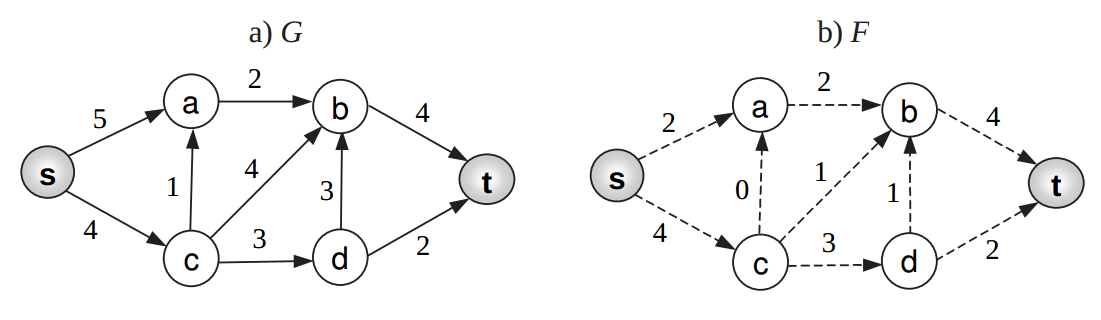
\includegraphics[width=0.8\linewidth]{/home/luigy/Escritorio/luigy_aed_2014/expo_fujos_maximos/info/figura.png}
	  \end{figure}
	\end{frame}

    %------------------------------------------------	

      
%------------------------------------------------
%------------------------------------------------
%------------------------------------------------
\section{Ejemplos}
%------------------------------------------------
%------------------------------------------------
%------------------------------------------------

	\begin{frame}
	  \begin{figure}
	    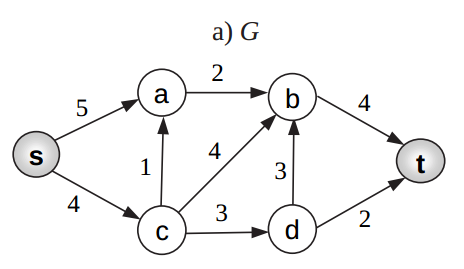
\includegraphics[width=0.8\linewidth]{/home/luigy/Escritorio/luigy_aed_2014/expo_fujos_maximos/info/1.png}
	  \end{figure}
	\end{frame}

    %------------------------------------------------	
    \begin{frame}
	  \begin{figure}
	    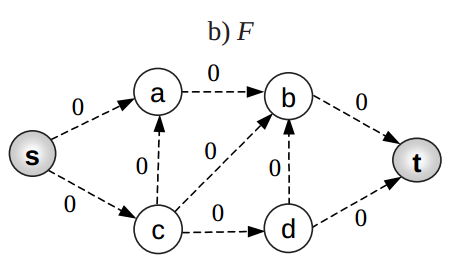
\includegraphics[width=0.8\linewidth]{/home/luigy/Escritorio/luigy_aed_2014/expo_fujos_maximos/info/2.png}
	  \end{figure}
	\end{frame}

    %------------------------------------------------	
    \begin{frame}
	  \begin{figure}
	    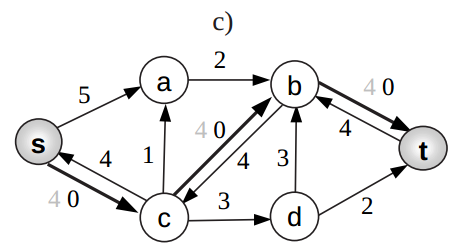
\includegraphics[width=0.8\linewidth]{/home/luigy/Escritorio/luigy_aed_2014/expo_fujos_maximos/info/3.png}
	  \end{figure}
	\end{frame}

    %------------------------------------------------	
    \begin{frame}
	  \begin{figure}
	    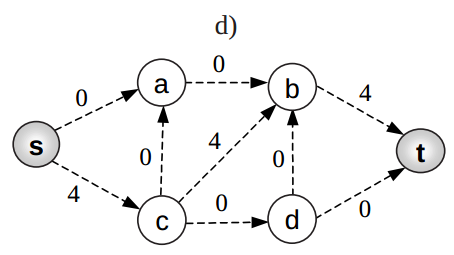
\includegraphics[width=0.8\linewidth]{/home/luigy/Escritorio/luigy_aed_2014/expo_fujos_maximos/info/4.png}
	  \end{figure}
	\end{frame}

    %------------------------------------------------	
    \begin{frame}
	  \begin{figure}
	    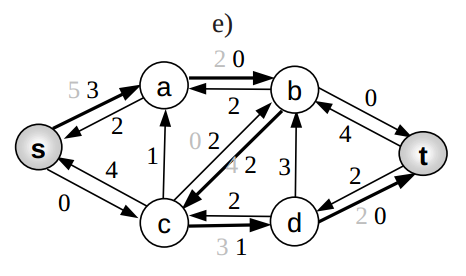
\includegraphics[width=0.8\linewidth]{/home/luigy/Escritorio/luigy_aed_2014/expo_fujos_maximos/info/5.png}
	  \end{figure}
	\end{frame}

    %------------------------------------------------	
    \begin{frame}
	  \begin{figure}
	    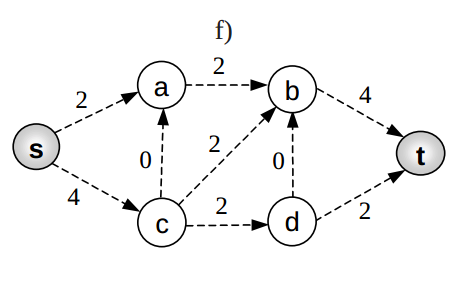
\includegraphics[width=0.8\linewidth]{/home/luigy/Escritorio/luigy_aed_2014/expo_fujos_maximos/info/6.png}
	  \end{figure}
	\end{frame}

    %------------------------------------------------	

	
%------------------------------------------------
%------------------------------------------------
%------------------------------------------------
\section{Aplicaci\'on}
%------------------------------------------------
%------------------------------------------------
%------------------------------------------------

  \begin{frame}
      \frametitle{Aplicaciones}
      \begin{itemize}
	\item Transporte de mercadería (logística)
	\item Flujo de gases y líquidos por tuberías
	\item Flujo de componentes o piezas en líneas de montaje
	\item Flujo de corriente en redes eléctricas
	\item Flujo de paquetes de información en redes de comunicaciones
	\item Tráfico ferroviario, etc.
      \item -----------
      
      \end{itemize}
      \end{frame}


      	
%------------------------------------------------
%------------------------------------------------
%------------------------------------------------
\section{References}
%------------------------------------------------
%------------------------------------------------
%------------------------------------------------

	%------------------------------------------------
	\begin{frame}
	\frametitle{References}
	  \footnotesize{
	    \begin{thebibliography}{99} % Beamer does not support BibTeX so references must be inserted manually as below
	    \bibitem[Smith, 2012]{p1} John Smith (2012)
	    \newblock Title of the publication
	    \newblock \emph{Journal Name} 12(3), 45 -- 678.
	    \end{thebibliography}
	  }
	\end{frame}

	%------------------------------------------------
	
	
%----------------------------------------------------------------------------------------

\end{document} 